In this section, I will describe and explain methods for performing LFC calibrations and RV extractions. I did not end up having access to star spectra with associated LFC exposures, such that I could calibrate the star spectra myself before computing the radial velocities. As a result, part one of the data analysis does not directly carry into part two, although, with the right data, it could.

\subsection{Calibration} 

    The calibration is needed to map each pixel on the CCD to a specific wavelength. Such a map is referred to as a wavelength solution. For this, we first shine a light source with known frequencies, preferably many discrete lines, onto the CCD. The pixels on the CCD on which each line appears can then be mapped to the known wavelength of the given line. EXPRES uses a Thorium Argon (ThAr) lamp with 4,000 lines across 82 orders for an initial rough wavelength solution. These values are then linearly interpolated to provide a wavelength solution for all pixels across the CCD. The data I have worked with came with this wavelength solution.
    
    For a better wavelength solution, EXPRES uses a laser frequency comb (LFC), which generates about 20,000 lines across 50 orders, with frequencies given by the relation

    \begin{equation}
        \label{eq:LFC_freq_eq}
        v_{n}=v_{\text{rep}} \times n+v_{\text{offset}}
    \end{equation}

    for integers $n$. The repetition rate $v_{\text {rep}}$ and offset frequency $v_{\text {offset }}$ are referenced against a GPS-disciplined quartz oscillator, providing calibration stability corresponding to a fractional uncertainty of less than $8 \times 10^{-12}$ for integration times greater than 1s\cite{first_RV_from_EXPRES}. The values I have used, $v_{\text{rep}} = 14e9$ and $v_{\text{offset}} = 6.19e9$, I found in the Excalibur github\cite{excalibur_github}.
    
    The following steps are followed to perform the LFC calibration: 1) determine the CCD pixel location of each LFC line, 2) use ThAr wavelength solution to find the corresponding mode $n$ in Eq. (\ref{eq:LFC_freq_eq}) to know the true wavelength of the line, and finally 3) find a way to estimate a wavelength solution in between LFC lines. 

    Figure \ref{fig:calib_illustration} is an illustration (not real data) of this process. The left panel shows LFC lines appearing in different locations on the CCD (with exaggerated variations and errors for clarity) and the corresponding wavelength solution on the y-axis given by Eq. (\ref{eq:LFC_freq_eq}). The middle and right panels illustrate two ways of modeling a wavelength solution in between LFC lines, polynomial fitting and cubic-spline interpolation respectively. With such a wavelength solution, you have a direct map between any location on the CCD (x-axis) and a wavelength solution (y-axis). This is to be performed in every order of the CCD.

    \begin{SCfigure}[1][!ht]%
        \begin{wide}  
            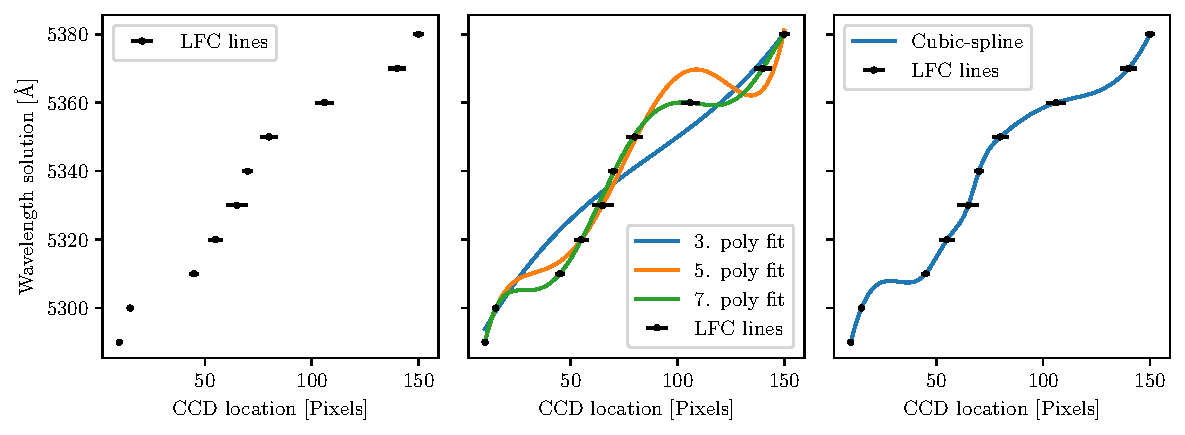
\includegraphics[width=\textwidth]{figures/calib/calib_illustration.pdf}
            \caption{Illustration of the LFC calibration process (not real data). See text for explanation.}
            \label{fig:calib_illustration}
        \end{wide}
    \end{SCfigure}

    \subsubsection{Determining LFC line locations}
    The right side of figure \ref{fig:LFC_CCD} shows an LFC exposure plotted in its entirety. It is clear that the LFC does not cover all orders of the CCD, but starts shortly before order 40 and stops around 76. To determine the location of the LFC lines I follow this procedure: 1) Find peaks using scipy peak finder, 2) make data slices around each peak with the size of the average distance between peaks, 3) using iminuit do a chi2 minimization fit to each peak with a super-Gaussian plus a linear background. See figure \ref{fig:LFC_CCD} left side.

    \begin{SCfigure}[1][!ht]%
        \begin{wide}  
            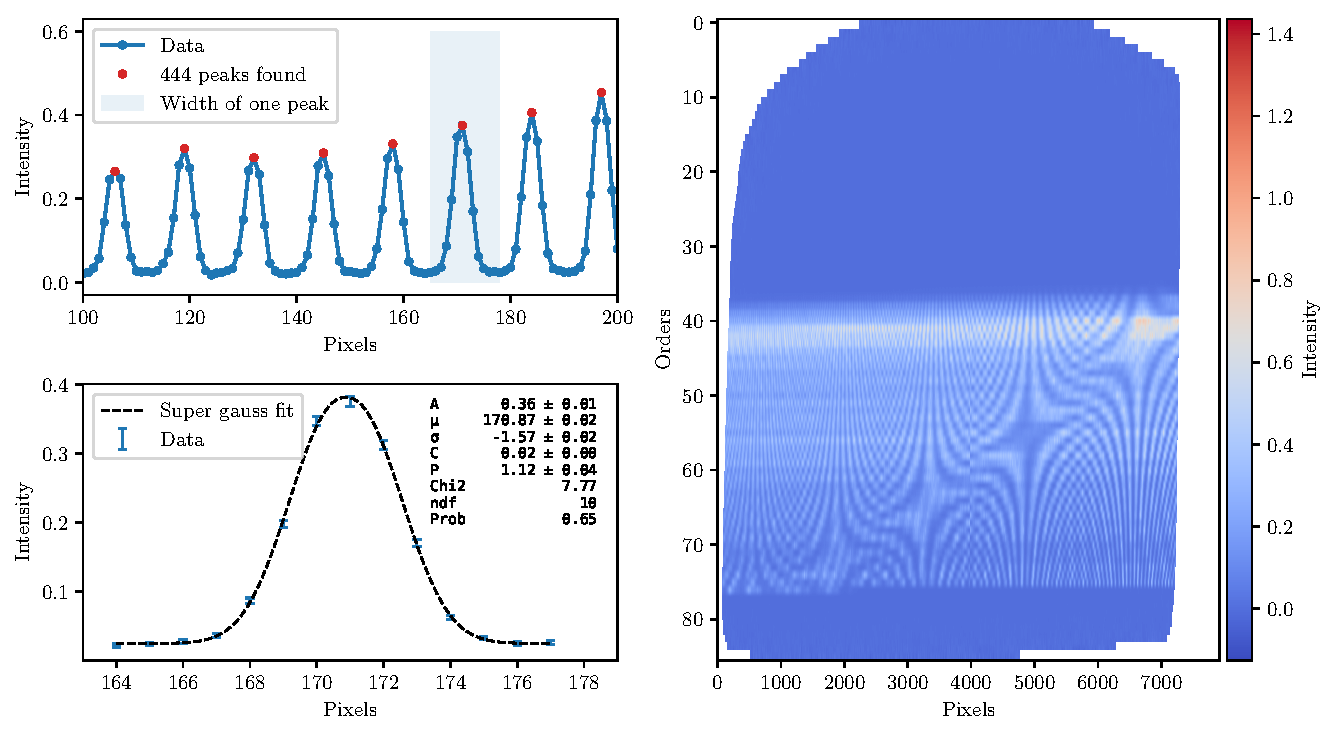
\includegraphics[width=\textwidth]{figures/LFC_peak_fitting_overview.pdf}
            \caption{Upper left: illustration of a few LFC lines in order 65. Peaks are identified with scipy peak finder. Lower left: each peak is fitted with a super gauss to find the exact top of the peak with uncertainties. Right: Measured intensities for the LFC across the CCD (unitless). }
            \label{fig:LFC_CCD}
        \end{wide}
    \end{SCfigure}

    A super-Gaussian, defined in Eq. (\ref{eq:LFC_super_gauss}), is a regular Gaussian but with an extra parameter, here denoted $P$, that allows the top of the Gaussian to be flattened. The last two terms here add a linear background and an offset.  
    
    \begin{equation}
        \label{eq:LFC_super_gauss}
        f(x ; A, B, C, P, \mu, \sigma) = A \exp \left(-\left(\frac{\left(x-\mu\right)^{2}}{2 \sigma^{2}}\right)^{P}\right) + B(x-\mu) + C
    \end{equation}

    The fit is then a standard chi2 minimization:

    \begin{equation}
        \label{eq:chi2_super_gauss}
        \chi^{2}=\sum_{i=1}^{N}\left[\frac{y_{i}-f(x ; A, B, C, P, \mu, \sigma)}{\sigma_{i}}\right]^{2},
    \end{equation}

    where $N$ is the number of data points, $x$ is pixel-space, $y_i$ and $\sigma_i$ are the measured intensity and uncertainty respectively. The fit returns the values and uncertainties for the parameters $A, B, C, P, \mu, \sigma$ when the chi2 is minimized.
    
    We are mainly interested in $\mu$, which gives the location of the LFC peak on the CCD (in pixel-space). With the initial rough wavelength solution derived from the ThAr lamp, I can determine what the approximate wavelength of the LFC peak should be. To find the better wavelength solution I then go look up the closest frequency given by Eq. (\ref{eq:LFC_freq_eq}), and we now have a map of ~20,000 points on the CCD with a good wavelength solution. 
    
    For a complete solution, we also need to estimate the wavelength solution between the LFC lines and to do that, I have explored two approaches: polynomial fitting and cubic-spline interpolation. Before moving on though, it is worthwhile to study the chi2 values from the many fits we just performed, as they can help us evaluate whether the errors of the original data are correct.

    \subsubsection{Errors in the calibration data}

    According to Zhao, the line-spread-function of EXPRES can best be represented by a super-Gaussian \cite{yale_data}, and so as we fit a super-Gaussian to the peaks, the chi2 will grow if the measured values do not agree with the predicted values within the uncertainties. For a given data point, if the measured value differs by exactly the uncertainty, that data point would contribute 1 to the sum. However, fitting with the super-Gaussian (including a linear background) we also have 6 fitting parameters that allow some wiggle room for the model to fit the data, which we must compensate for. For a given data series, such as an LFC peak, we can expect the chi2 to roughly equal the number of data points in the sum \emph{minus} the number of parameters in the fit, i.e. the number of the degrees of freedom:
    
    \begin{equation}
        \label{eq:ndof}
        N_\text{dof} = N_\text{data-points} - N_\text{fit-parameters} =  13 - 6 = 7,
    \end{equation}

    as I use roughly 13 data points in each fit (the LFC line spacing does vary a bit across the CCD). 

    So if we plot all chi2 values we get from fitting the LFC lines, as I have done in figure \ref{fig:calib_errors}, we should see a typical chi2 distribution with a peak around 7. Using the uncertainties as provided in the data file, the chi2 distribution is however very flat (blue curve). It peaks somewhere around 25, which suggests that the uncertainties are about a factor $\sqrt{3}$ too small (square-root because the chi2 of course is squared and $25/3 \sim 8$). Multiplying the uncertainties by $\sqrt{3}$ and fitting the peaks again gives a chi2-distribution with a peak roughly around 7-8 (green curve).
                
    \begin{SCfigure}[1][!ht]%
        \begin{wide}  
            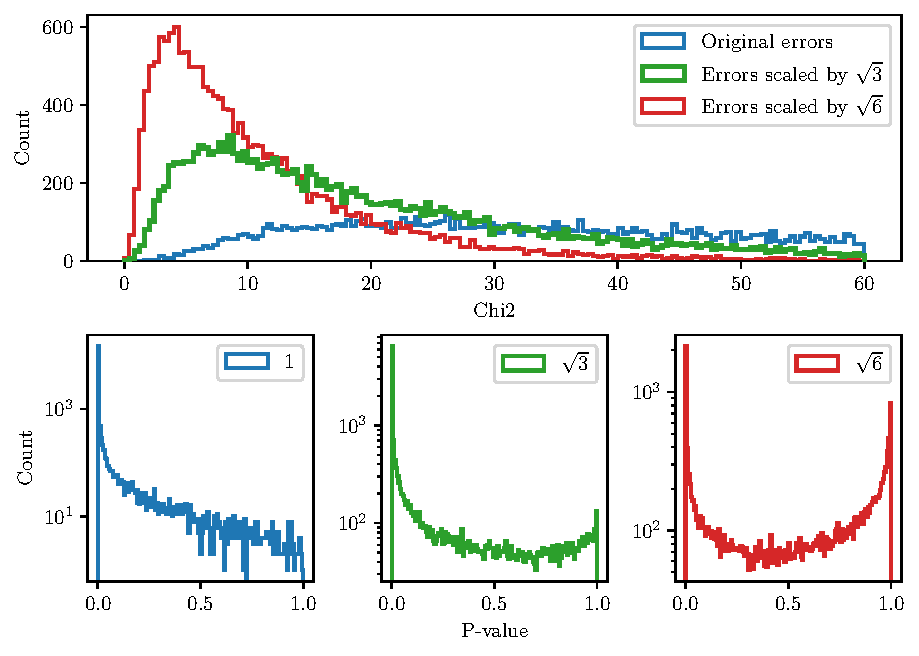
\includegraphics[width=\textwidth]{figures/calib/calib_errors2.pdf}
            \caption{Chi2-values and p-values from individual LFC peak super-Gaussian fits with errors multiplied by different scale-factors (1, $\sqrt{3}$ and $\sqrt{6}$).}
        \label{fig:calib_errors}
        \end{wide}
    \end{SCfigure}

    Additionally, we can also look at the distribution of the p-values. With proper uncertainties, we should expect neither too many awful fits (p=0) nor too many perfect fits (p=1), but rather a roughly flat distribution. Although the chi2-distribution check is more clear-cut, the p-value distribution for uncertainties scaled by $\sqrt{3}$ (green) is better. Scaling by $\sqrt{6}$ is too much: the chi2 peaks around 4 and the p-distribution shows many more perfect fits.

    \subsubsection{Poly-fit calibration}
    Since the LFC peak locations, as seen in the right plot in figure \ref{fig:LFC_CCD}, appear to exhibit a certain periodic behavior, my initial approach to compute a wavelength solution between LFC lines was to fit the LFC peak locations with a polynomial. Looking at the residuals of fitting the LFC line locations with polynomials of increasing degree revealed smaller and smaller periodic variations, until reaching 5th degree, see figure \ref{fig:LFC_calib_poly_degrees}. The p-value drops to 0 for 6th degree, and the per-line rms (given by Eq. (\ref{eq:line_rms})) explodes. Only LFC lines with a chi2 (from the super-Gaussian fit) smaller than 100 were used for the analysis and errors were scaled by $\sqrt{3}$.

    The residuals plotted in figure \ref{fig:LFC_calib_poly_degrees} show the difference between the theoretical wavelength for each LFC line (Eq. (\ref{eq:LFC_freq_eq})) and the wavelength that the calibration predicts for that location. You can get a feel for the quality of the calibration by looking at the residuals, but a more formal quantification is to compute the per-line rms for a given LFC exposure as: 
    
    \vspace{0.15cm}

    \begin{equation}        
        \text{RMS/line } [\text{ms}^{-1}] = \sqrt{\sum_{n=1}^{N} \frac{\left[\frac{\left(\lambda_{n, \text {pred.}}-\lambda_{n, \text {theory}}\right)}{\lambda_{n,\text{theory}}} \times c\right]^{2}}{N}}
        \label{eq:line_rms}
    \end{equation}
    
    \vspace{0.25cm}

    for $N$ lines, where $c$ is the speed of light in m/s.
    
    \begin{SCfigure}[1][!ht]%
        \begin{wide}  
            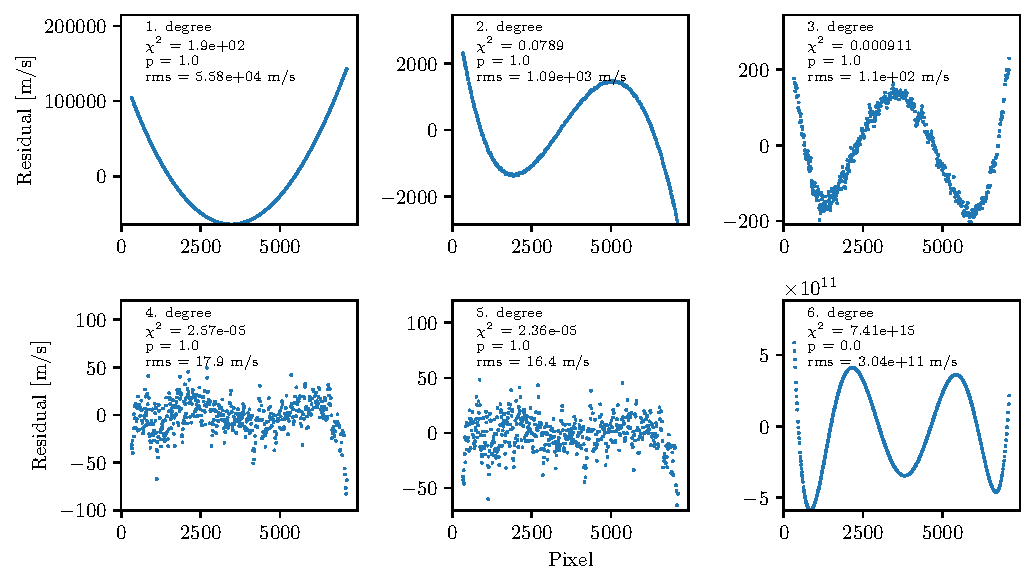
\includegraphics[width=\textwidth]{figures/calib/calib_poly_fit_degrees_order44_residuals_ang.pdf}
            \caption{Example of residuals from fitting LFC line locations with polynomials of increasing degree in one order (44). The x-axis shows pixels and the y-axis residuals in m/s in all plots. Errors used for determining line locations have been scaled by $\sqrt{3}$. The noted rms in each plot is the per-line rms as defined in Eq. (\ref{eq:line_rms}).}
            \label{fig:LFC_calib_poly_degrees}
        \end{wide}
    \end{SCfigure}

    \subsubsection{Interpolation calibration}
    Although there are large periodic trends in the residuals in figure \ref{fig:LFC_calib_poly_degrees}, on the very small scale, the changes seem rather random. A better approach might therefore be to use interpolation, as this is more flexible and copes better with very complicated and non-repetitive behavior.
    
    A cubic-spline interpolation would force all the residuals to be zero, so to evaluate the method, we can interpolate all the even peaks and compute the residuals for the odd peaks. Then flip around to interpolate the odd peaks and compute the residuals for the even peaks.

    Figure \ref{fig:calib_poly_vs_interp} shows a comparison of the residuals from a 5th degree poly-fit and the cubic-spline. For the cubic-spline I get a per-line rms of 10.0 m/s, while the poly-fit gives $5.73 \times 10^8$ m/s, which suggests that the cubic-spline approach is the better one. It is also worth noting that because the interpolation was done on only half the data points at a time, it will be even better when performed on all data points, as it would be when used for calibrating data before an RV analysis.

    \begin{SCfigure}[1][!ht]%
        \begin{wide}  
            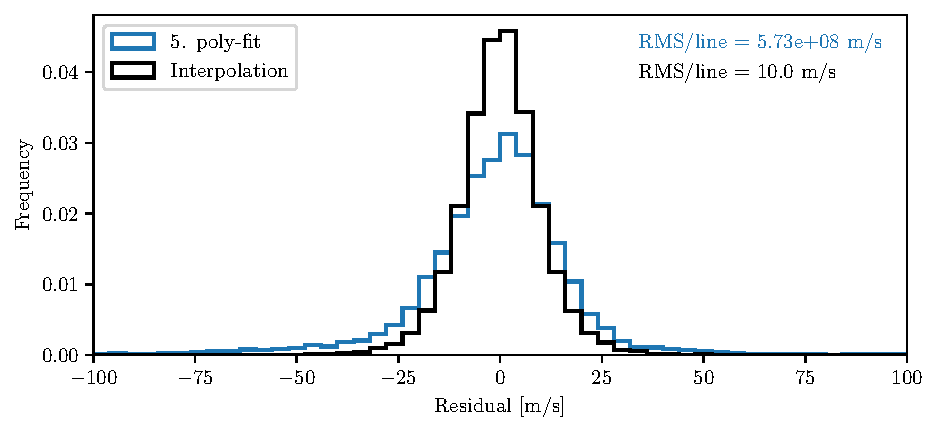
\includegraphics[width=\textwidth]{figures/calib/hist_peak_residuals_poly_and_interp.pdf}
            \caption{Residuals from calibrations performed through a 5th degree poly-fit and a cubic-spline interpolation. The per-line rms as defined in Eq. (\ref{eq:line_rms}) is given in the top-right corner in the color of the corresponding method.}
            \label{fig:calib_poly_vs_interp}
        \end{wide}
    \end{SCfigure}

\subsection{Radial velocity extraction}

    To extract radial velocities we need to measure the Doppler shift between spectra from different days of observation. One way to do that is to compute the cross-correlation, which is a measure of the similarity of two data series as a function of the displacement of one relative to the other.
    
    We can do this either for individual absorption features, chunks of the spectrum a few angstroms wide, or entire orders at a time. I have chosen primarily to work with the individual features.

    Due to a lack of access to data consisting of star spectra with associated LFC captures, I have worked on RV extractions using already calibrated data provided by Zhao. This data has been calibrated using a technique called Excalibur \cite{zhao2021excalibur}.
    
    The data is visualized in \ref{fig:rv_data_overview}, where the top left shows an extract of wavelength vs. intensity data from an observation of HD 34411. The file also includes a model of the continuum function, with which we can normalize the spectrum through division, shown in the bottom left. Plotted on the right side are all continuum normalized data within the EXCALIBUR mask, i.e. data marked as having a proper calibration.

    \begin{SCfigure}[1][!ht]%
        \begin{wide}  
            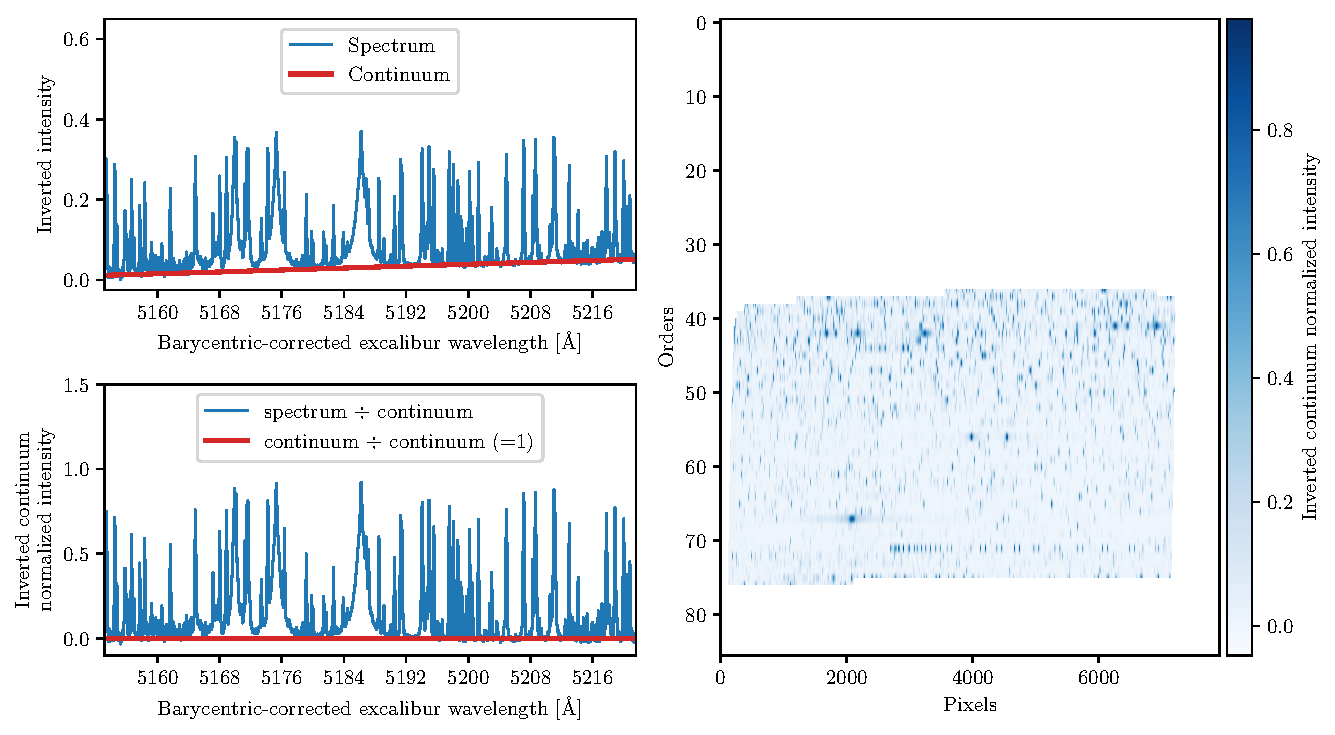
\includegraphics[width=\textwidth]{figures/rv_data_overview.pdf}
            \caption{Overview of Excalibur calibrated data from an observation of HD 34411. Upper left: extract of wavelength solution vs. intensity. Lower left: continuum normalized spectrum. Right: all continuum normalized data within the Excalibur mask.}
            \label{fig:rv_data_overview}
        \end{wide}
    \end{SCfigure}
            
    \subsubsection{Finding and matching features across observations}

    To measure how much individual absorption features move in between observations, the first challenge is to find the "same" features in both observations. To do that, I have devised the following procedure:
    
    \begin{itemize}
        \item Load intensities from the data column \verb|"spectrum"| and errors from \verb|"uncertainty"| as well as Excalibur calibrated barycentric-corrected wavelengths from \verb|"bary_excalibur"|, all masked by \verb|"excalibur_mask"|.
        \item Normalize intensities and errors with the continuum function from \verb|"continuum"|.
        \item Invert intensities to turn absorption features into positive peaks by $y = 1 - y$.
        \item Locate peaks using \verb|find_peaks| from \verb|scipy.signal| with minimum peak distance of 5 pixels and a minimum peak prominence of 0.25 (unitless).
        \item Finally slice data around each peak with a width of 30 data points. 
    \end{itemize}

    And then to match features/peaks between two observations:

    \begin{itemize}
        \item Iterating through the peaks of observation1, for each peak, find the closest peak in observation2. With Excalibur calibrated data, peaks should not shift so much that they overlap. However, the algorithm laid out so far does sometimes match peaks that are far apart or do not resemble each other in shape at all. To bypass such matches we can add two filters:
        \begin{itemize}
            \item Maximum peak distance: We could filter out all matches where the distance between the peaks is equivalent to a radial velocity greater than 12.5 m/s (the RV Jupiter induces in the Sun). However, since we are dealing with discrete data, the difference sometimes comes out much larger than it really is and a narrow cut of 12.5 m/s would remove many good matches. Instead, setting a very generous cut of 0.5 Å, equivalent to about 20-30 km/s depending on the wavelength, filters out the few very bad matches, but leaves the rest. When analyzing non-barycentric-corrected data, I set this up to 1Å. 
            
            \item Maximum difference between the areas under the graph of two features (the sum of the intensity values in the feature): Peaks with similar shapes will give a low difference. This filter is most useful when analyzing non-barycentric-corrected, where features often move so much that they overlap. Figure \ref{fig:good_match_bad_match} shows an example of a bad and a good match, where the bad match can be avoided by setting the max area difference down to 0.1 (unitless). 
        \end{itemize}
        \item A way to formally select the best values for these filters is yet to be worked out.
    \end{itemize}

    % \begin{SCfigure}[1][!ht]%
    %     \begin{wide}  
    %         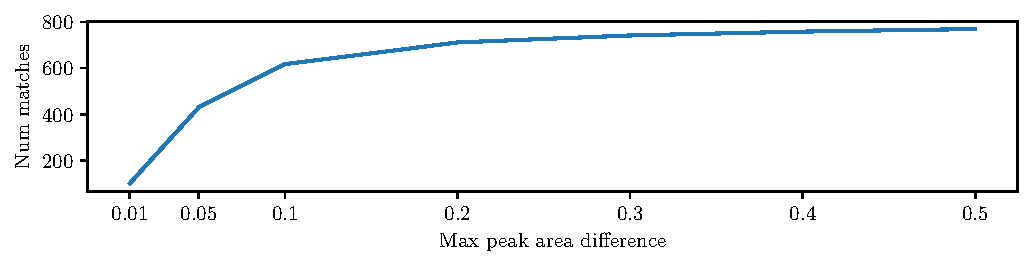
\includegraphics[width=\textwidth]{figures/max_peak_area_diff_vs_Nmatches.pdf}
    %         \caption{Average number of matches found as a function of max peak area difference for all features in observations for HD 34411.}
    %         \label{fig:max_area_diff_vs_n_matches}
    %     \end{wide}
    % \end{SCfigure}

    \begin{SCfigure}[1][!ht]%
        \begin{wide}  
            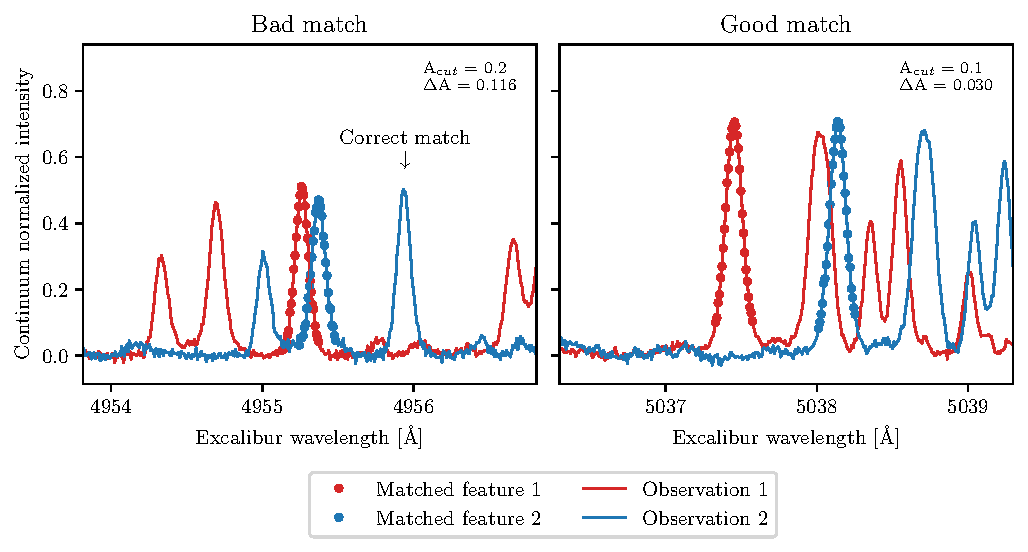
\includegraphics[width=\textwidth]{figures/good_match_bad_match.pdf}
            \caption{Example of match filtering with non-barycentric-corrected data, where features move a lot. The maximum area difference cut was set to 0.2 and 0.1 on the left and right plots respectively. The cut on the left plot was not strict enough to avoid the bad match that was made, with an area difference of 0.116. While on the right plot, the correct feature was selected spite another feature being closer in wavelength.}
            \label{fig:good_match_bad_match}
        \end{wide}
    \end{SCfigure}

    \subsubsection{Computing velocity shift as the cross-correlation}

    At this point, I have a list of matching features in different observations. We can now compute the cross-correlation for each match as a chi2 minimization fit with the radial velocity as our fit parameter. The fit will converge when it has found the radial velocity that shifts one peak onto the other one.
    
    Before moving on though, we have to cubic-spline interpolate the spectra data. This is needed for two reasons: 1) The shifts we are looking for are much smaller than the individual pixels on the CCD, so we need to be able to shift by sub-pixel amounts, and 2) to compute the difference in intensity values between peaks, the intensity values must have the same wavelength solution, but, since EXPRES is calibrated independently for each observation, the wavelength solutions are different.
    
    So I cubic-spline interpolate the spectra data from the first observation in the match, but before interpolating the second observation, I shift the wavelength solution by multiplying the shift factor from Eq. (\ref{eq:our_doppler}). Now I can evaluate the two interpolation functions on a common wavelength range, using $N=1000$ steps\footnote{1000 steps appeared as the best balance between run time and resulting uncertainty. See figure \ref{fig:err_vs_run_time} in appendix \ref{appendix:RV_extraction}}, and I am ready to compute the chi2:
        
    \begin{equation}
        \label{eq:shift_fit_chi2}
        \chi^{2}=\sum_{i=1}^{N}\left[\frac{y_{i}-f(x; v)}{\sigma_{i}}\right]^{2}
    \end{equation}
    
    where $y_i$ are the unshifted interpolated intensities from the first observation, $\sigma_i$ the errors on the intensity of the first observation also sampled through a cubic-spline interpolation, and the function $f(x; v)$ is the cubic-spline interpolation function given by interpolating the intensity values of the second observation with wavelength values shifted by Eq. (\ref{eq:our_doppler}), evaluated on the wavelength range common to both features: 
    
    \begin{equation}
        f(x; v) = \textbf{interp}[x \times ( 1 + v/c), y]\,(x_\text{common})
    \end{equation}
    
    I then compute the cross-correlation and obtain the radial velocity, $v$, as a minimization of Eq. (\ref{eq:shift_fit_chi2}) using iminuit.
    
    \subsubsection{Computing velocity shifts for all features}

    We can now find and compute the cross-correlation for all feature matches between two observations. In general, I find between 500-1000 matches between two observations, which results in a fair amount of statistics. The computed radial velocities do build up a normal distribution around a central value, but there are many outliers. This is due to primarily two things: 1) Bad matches making it through the selection filters, and 2) stellar activity.
    
    A better matching algorithm could supposedly be developed, but for now, I have just experimented with setting different cuts both in radial velocity and chi2 to weed out the bad ones. What I have found to work the best however is simply taking the median instead of the weighted average or the mean, as the median is much less affected by outliers. And as there is no reason to believe that stellar activity would cause more RV outliers in one particular direction, so the spread can be assumed to be symmetric, and the median is thus a good approximation. Figure \ref{fig:median-mean-weighted-average} shows an example of computed radial velocitiy shifts for all features between two observations. It is clear that neither the weighted average (yellow) nor the regular mean (black) are good approximations of the total shift. The median (red), however, does a good job. 
    
    We also see a constellation of features likely to be affected by stellar activity on the far right, and a match on the left, which appears bad, but actually turns out to be "correct", but of a an absorption line so broad that the data-slice does not have enough information for the fit to converge properly (plotted in figure \ref{fig:bad_match_example} in appendix \ref{appendix:RV_extraction}).

    \begin{SCfigure}[1][!ht]%
        \begin{wide}  
            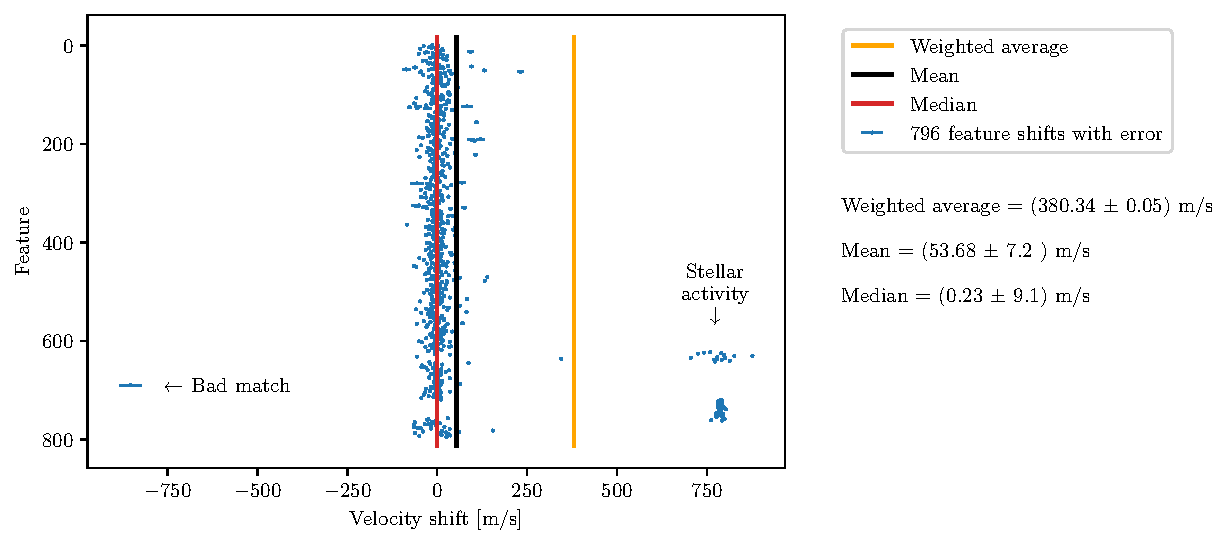
\includegraphics[width=\textwidth]{figures/median-mean-weighted.pdf}
            \caption{Comparison of weighted average, mean and median for computed rv shifts for two observations of HD 34411. The feature on the left side turns out to be a very broad feature, for which the standard data slice is too narrow and therefore yields bad results, (see figure \ref{fig:bad_match_example} in appendix \ref{appendix:RV_extraction}) for details. While the features on the right side are likely to be caused by some kind of stellar activity.}
        \label{fig:median-mean-weighted-average}
        \end{wide}
    \end{SCfigure}

    Also plotted in figure \ref{fig:median-mean-weighted-average} are the respective errors on the weighted average, the mean, and the median. As it is the median that I have decided to work with, it would make sense to use the median error, 
    
    $$
        \sigma_{\text{median}} = \frac{\sigma}{\sqrt{N-1}} \times \sqrt{\pi/2},
    $$
    
    for large $N$, where $\sigma$ is the standard deviation, however, it not only comes out very large but also breaks the propagation of the original errors from the spectrograph. The weighted error carries on the information of the original errors, but it comes out very small. For the sake of continuing with the analysis, I will go on with the weighted error however.
    
    \subsubsection{Extracting relative shifts from an overconstrained system}
    
    With the devised method we can now compute the relative radial velocity shift between two observations and get out one number with an uncertainty. The next most obvious step would be to compute the shift between observations 1 and 2, 2 and 3, etc. Doing this however leads to correlated results, as the difference between say observations 1 and 10 would depend on all the observations in between, and if there is one bad one, it will affect all the rest. To circumvent this, we can first compute the relative shift between all observations. This will give us an \emph{overconstrained system}, in the sense that there is more information than necessary. All these differences can then be reduced down to a single array, where each shift is relative to all the rest, not only the neighbor. 
    
    Computing the shifts between all observations yields an $N\times N$ upper triangular matrix, where each cell is the shift between observations $i$ and $j$, and thus with a diagonal of zero. I will call this matrix $\Delta V_r^{ij}$, see figure \ref{fig:shift_matrix} for an example.
    
    \begin{SCfigure}[1][!ht]%
        \begin{wide}  
            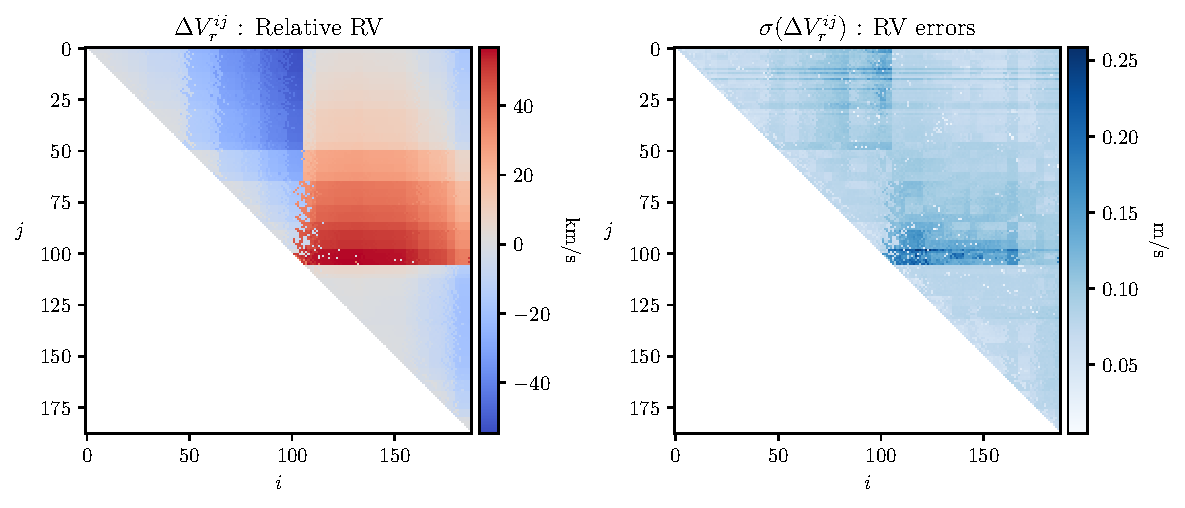
\includegraphics[width=\textwidth]{figures/shfits_matrix_non_bary.pdf}
            \caption{Radial velocity shifts matrix computed for 188 observations for HD34411 using Excalibur calibrated but non-barycentric-corrected data (column \texttt{excalibur}). Each cell shows the median radial velocity shift for all features found between observations $i$ and $j$.}
        \label{fig:shift_matrix}
        \end{wide}
    \end{SCfigure}

    \vspace*{-0.5cm}
            
    To reduce the matrix to one array, we can perform another chi2 minimization fit, defined bellow in Eq. (\ref{eq:matrix_reduction_fit}), in which we fit an array of parameters we can call $V_r^i$ of length $N$ (the number of observations), initialized to zero. The chi2 will be at its minimum when it has found an array of velocities $V_r^i$ that best describe all the differences in the matrix $\Delta V_r^{ij}$ and each of the resulting velocities are thus relative not only to its neighbors but to all the other observations as well, thereby avoiding the correlation.
    
    \begin{equation}
        \label{eq:matrix_reduction_fit}
        \chi^{2}=\sum_{i,j = 0}^{N}\left[\frac{ \Delta V_{r}^{ij} - (V_r^i - V_r^j) }{\sigma(\Delta V_{r}^{ij})}\right]^{2} \quad : \quad i < j.
    \end{equation}

    To test the method, I have analyzed non-barycentric-corrected data. The resulting $\Delta V_r^{ij}$ matrix is the one plotted in figure \ref{fig:shift_matrix} while the extracted relative radial velocities (the fit parameters $V_r^i$) are plotted in figure \ref{fig:RV_results_non_barycentric} (black), where we see a clear signal of Earth's movement. I have fitted the data with a periodic function and found a  period of $(366.482 \pm 3\mathrm{e}{-6})$ days and an amplitude of $(28.132 \pm 9\mathrm{e}{-7})$ km/s. This is very close to the actual orbital speed of the Earth, although we should not expect that, as the star is unlikely to lie in the plane of the Earth's orbit. There are however three other things to notice: 1) the error of the period does not cover the discrepancy with the actual value of 365.24 days, 2) the very high chi2 value, and 3) the p-value of zero. These suggest very clearly that my errors are wrong. Nevertheless, the signal is clear and the period found is definitely on the right order of magnitude, from which I confirm that my method, in general, is working. The direct velocity shifts between observations 1 and 2, 2 and 3, etc.,  are plotted in blue in figure \ref{fig:RV_results_non_barycentric}, and it is clear that the last step of computing the relative shift between all observations is vital.

    \begin{SCfigure}[1][!ht]%
        \begin{wide}  
            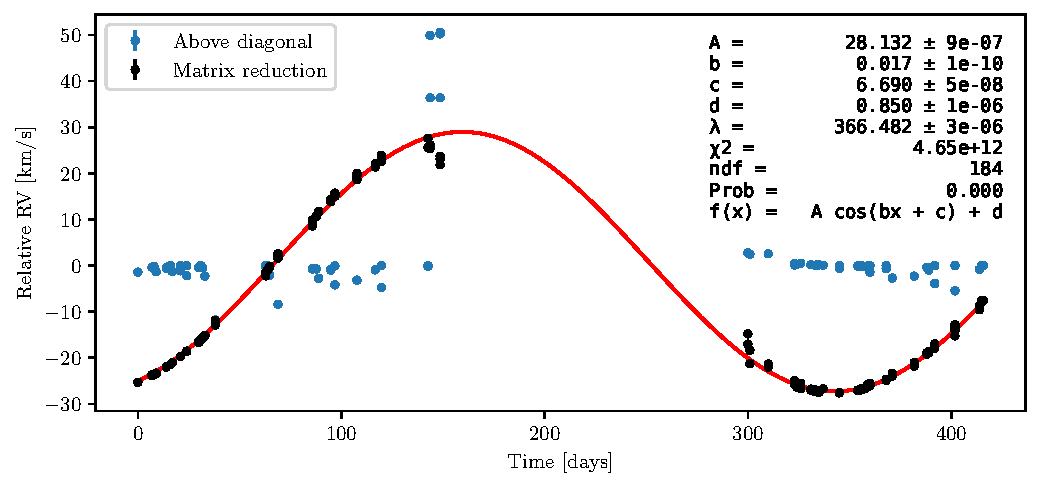
\includegraphics[width=\textwidth]{figures/shift_non_bary_centric.pdf}
            \caption{Final relative radial velocity results for 188 observations of HD 34411 using Excalibur calibrated but non-barycentric-corrected data (data column \texttt{excalibur}). Black: values computed through the overconstrained system approach. Blue: above diagonal of $V_r^{ij}$.}
            \label{fig:RV_results_non_barycentric}
        \end{wide}
    \end{SCfigure}


    Although the number of computations necessary for the described analysis is high, it is possible to run for 188 observations on a powerful laptop in about 2 hours. More run-times are listed in appendix \ref{appendix:RV_extraction}. The implementation of the described methods is hosted on GitHub\footnote{\href{https://github.com/Harteg/LFC-calibration-RV-extractions}{\textit{https://github.com/Harteg/LFC-calibration-RV-extractions}}}. 

    
    

